\documentclass[a4paper,12pt, titlepage]{article} 
% пакет для задания полей страницы командой \geometry :
\usepackage{geometry}
\geometry{left=3cm,right=1.5cm,top=2cm,bottom=2cm}
\usepackage[utf8]{inputenc}
\usepackage[english,russian]{babel}
\usepackage{amsmath}
%\usepackage{amsthm}
%\usepackage{cmap}
\usepackage{indentfirst}
\usepackage{a4wide,amssymb}
%\usepackage[pdftex]{graphicx}
%\usepackage[pdftex]{graphics}
%\usepackage{wrapfig}
%\linespread{1.3}               % полтора интервала. Если 1.6, то два интервала
\pagestyle{plain}               % номерует страницы

\usepackage{graphicx}
\renewcommand{\topfraction}{1}
\renewcommand{\textfraction}{0}

% The following code enables back references:
\usepackage{color} 
\definecolor{darkgreen}{rgb}{0,.5,0} 
\usepackage[unicode,colorlinks,filecolor=blue,citecolor=darkgreen,pagebackref]
{hyperref}


%opening
\title{Восстановление многогранника по набору его теневых контуров \\ Обзор
материалов и план работы}
\author{Палачев Илья}

\begin{document}

\maketitle

\tableofcontents

\newpage
\section{Постановка задачи}

Имеется некоторый физический камень, геометрическая форма которого
представляет собой многогранник. Имеется установка, которая позволяет получать
информацию о его форме следующим образом:
 
\begin{enumerate}
  \item Камень жестко закрепляется одной своей гранью на горизонтальной
  подставке.
  \item Производится фотографирование камня вдоль некоторого фиксированного
  горизонтального направления $\nu_{0}$.
  \item Результатом фотографирования является монохромное изображение без
  каких-либо внутренних ребер, иными словами, "тень" камня.
  \item Затем подставка вместе с закрепленным на ней камнем поворачивается на
  фиксированный угол $\alpha_{0}$ в горизонтальной плоскости и процесс
  повторяется начиная с пункта 2.
\end{enumerate}
 
Этот процесс повторяется $K = \frac{2 \pi}{\alpha_{0}}$ раз, пока не получатся
фотографии камня по всем направлениям $\alpha_{k} = k \alpha_{0}$, где
$k = 1, 2, \ldots, K$. Все эти фотографии подвергаются обработке, в результате
которых получаются так называемые \textbf{теневые контуры} -- многоугольники,
лежащие в плоскостях, ортогональных горизонтальным векторам, образующим углы
$\alpha_{k} = k \alpha_{0}$ с осью $Ox$. 

Требуется построить трехмерный многогранник, форма которого наилучшим образом
соответствует исходному камню. При этом под качеством построенной модели
подразумевается следующее:

\begin{enumerate}
 \item Тени модельного многогранника наилучшим образом приближают тени,
 полученные из измерений.
 \item В многограннике характерные вершины и грани не разделены на несколько
 вершин и граней.
\end{enumerate}

\newpage
\section{Исторический обзор смежных вопросов}

Далее приводится обзор некоторых статей, которые были написаны в целях решения
задач, схожих с рассматриваемой. Как оказалось, особенно большое сходство было
найдено с задачей оценки опорной функции в геометрической томографии. В целях
последовательности изложения сначала приводится понятие опорной функции, а
затем задачи и алгоритмы их решения.

\subsection{Понятие опорной функции выпуклого тела}

Для простоты будем рассматривать выпуклые тела в трехмерном пространстве
$\mathbb{R}^{3}$, содержащие в своей внутренности начало координат $O$.
Для некоторых понятий будем давать определения и формулировки для случая
произвольной конечной размерности.

Как известно, выпуклое тело можно однозначно представить как пересечение 
полупространств всех его касательных плоскостей 
$K = \bigcap \limits_{x \in K} R_{x}$, где $R_{x}$ -- то из двух
полупространств, на которые плоскость $\pi_{x}$, касательная к телу $K$ в
точке $x$, делит $\mathbb{R}^{3}$, которое содержит в себе целиком все тело
$K$. Всякому выпуклому телу можно поставить в соответствие набор касательных 
плоскостей $\pi_{x}$, по которым его можно построить. Обратное неверно: не
всякому произвольному набору плоскостей можно поставить в соответствие тело,
касающееся всех этих плоскостей.

Всякую касательную плоскость $\pi_{x}$ можно однозначно охарактеризовать
единичным вектором нормали $u_{x}$ и расстоянием $h_{x}$ от начала координат 
$O$ до плоскости. Поскольку две разные касательные плоскости не могут иметь
одинаковые векторы нормалей, то можно рассматривать множество всех касательных
плоскостей выпуклого тела как функцию, определенную на всех единичных векторах
$u \in S_{2}$:

$$h_{K}: S^{2} \to \mathbb{R}_{+}$$

Более общее понятие включающее в себя выше указанное было введено в 1903 году
Минковским.

\begin{flushleft}
\textbf{Определение}. Будем называть \textbf{опорной функцией} выпуклого тела
$K \subset \mathbb{R}^{n}$ следующую функцию 
$h_{K}: \mathbb{R}^{n} \to \mathbb{R}_{+}$:

$$h_{K}(u) = \max \limits_{x \in K}(x, u)$$
\end{flushleft}

Если взять некоторую точку $u_{0}$ на единичной сфере $S^{n - 1}$, и вычислить
в ней значение опорной функции $h_{K}(u_{0})$, то по этим данным можно
построить касательную плоскость к выпуклому телу в некоторой (неизвестной!)
точке $x \in K$. Такую плоскость (в контексте, когда нет информации о положении
точки касания) принято называть опорной плоскостью.

\begin{flushleft}
 \textbf{Определение}. \textbf{Опорной плоскотью} выпуклого тела $K$ по
 направлению $u \in S^{n - 1}$ называется плоскость с нормалью $u$, расстояние
 от которой до начала координат равно $h_{K}(u)$
\end{flushleft}

Очевидно, что опорная функция выпуклого тела обладает следующим свойством:

$$h_{K}(\lambda u) = \lambda h_{K}(u)$$

Следовательно, для практики достаточно иметь дело только с ограничением опорной
функции на единичную сферу. В статье \cite{journals/jmiv/KarlKVW96} вводится
понятие \textbf{приведенной опорной функции}:

$$H_{K} (u) = h_{K} (\frac{u}{||u||})$$

которая в действительности педставляет собой расстояние от начала координат
$\mathbb{O}$ до опорной гиперплоскости по направлению $u$.

Более подробно свойства опрной функции рассматриваются в статье
\cite{journals/cviu/GhoshK98}.

%(TODO: прочесть и законспектировать)

\newpage
\subsection{Восстановление выпуклого многоугольника по измерениям его опорной
функции (по статье Prince, Willsky)}

\subsubsection{Постановка задачи и основные определения}

В работе \cite[Prince - Willsky (1990)]{journals/pami/PrinceW90}
рассматриваются алгоритмы для восстановления \textbf{двумерных} выпуклых тел по
измерениям их опорных функций. Изначально изучение данной проблемы было
мотивировано задачей из компьютерной томографии. А именно, в томографии
делаются измерения интегралов плотности поглощения излучения объектом вдоль
различных фиксированных прямых. Допустим, что известны интегралы плотности
поглощения по пучку прямых $L(t, \theta)$, где угол $\theta$ фиксирован. Тогда
по этой информации можно определить положение двух опорных прямых к данному
объекту (см. рис. \ref{tomography-application}).

\begin{figure}[ht]
    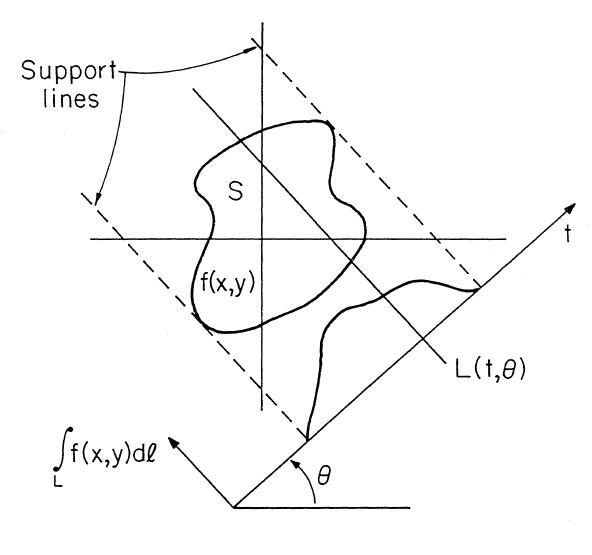
\includegraphics[width=10cm]{images/tomography-application.jpg}
    \caption{Граница носителя функции плотности поглощения определяет две
    опорные прямые к объекту}
    \label{tomography-application}
\end{figure}

По имеющимся измерениям опорной функции можно потроить грубое приближение
расмматриваемого тела -- путем обыкновенного пересечения полуплоскостей,
соответствующих опорным прямым. Однако на практике измерения подвержены
ошибкам и известны лишь с некоторой точностью. Так, может оказаться, что
после пересечения построенное тело будет касаться не всех заданных прямых.
Это приводит к тому, что всего одно грубое измеренние может заблокировать
воздействие других (более точных) измерений на результат (см. рис.
\ref{inconsistent}).

\begin{figure}[ht]
    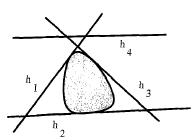
\includegraphics[width=10cm]{images/inconsistent-support-planes.jpg}
    \caption{В случае неточных измерений опорной функции тело нельзя строить
    как пересечение полупространств}
    \label{inconsistent}
\end{figure}

Prince и Willsky рассматривают в своей статье случай, когда измерения опорной
функции получаются по фиксированному набору направлений

$$u_{i} = (cos \theta_{i}, sin \theta_{i})$$

где углы $\theta_{i}$ берутся по всему отрезку $[0, 2 \pi]$ с постоянным шагом:

$$\theta_{i} = i \cdot \Delta \theta$$

где $\Delta \theta = \frac{2 \pi}{M}, i = 0, \ldots, M - 1, M \leq 5$. Более
общий случай, когда направления измерений выбираются произвольным образом,
описывается в статье
\cite[Lele - Kulkarni - Willsky (1992)]{journals/josaa/LeleKW92}.

\subsubsection{Критерий согласованности набора опорных чисел}

Ключевым понятием в статье является следующее

\begin{flushleft}
 \textbf{Определение}. \textbf{Набором опорных чисел}
 $(h_{0}, h_{1}, \ldots, h_{M - 1})^{T}$выпуклого тела $K$ по заданному набору
 направлений $u_{i}, i = 0, \ldots, M - 1$ называется называется вектор в
 $\mathbb{R}^{M}$, составленный из значений опорной функции по соответствующим
 направлениям: $(h_{K}(u_{0}), h_{K}(u_{1}), \ldots, h_{K}(u_{M - 1}))^{T}$.
\end{flushleft}

Вектор, составленный из набора опорных чисел, является по сути аналогом
непрерывной опорной функции. Если говорить более точно, опорный вектор есть
сеточная функция, соответствующая непрерывной функции $h(\theta)$. Всякая ли
непрерывная функция является опорной функцией некоторого выпуклого тела? Ответ
на этот вопрос дает следующая теорема:

\begin{flushleft}
 \textbf{Теорема 1}. \textbf{Критерий опорной функции}.
 
 Непрерывная функция $h : \mathbb{R} \to \mathbb{R}_{+}$ является опорной
 функцией некоторого выпуклого тела тогда и только тогда, когда для всех
 $\theta \in \mathbb{R}$ выполнено следующее неравенство:
 
 $$
 h''(\theta) + h(\theta) \geq 0
 $$
\end{flushleft}


Основным теоретическим результатом статьи, на котором основаны все алгоритмы,
является следующая

\begin{flushleft}
 \textbf{Теорема 2}. \textbf{Опорная теорема}

  Набор действительных чисел $h \in \mathbb{R}^{M}, M \leq 5$ является набором
  опорных чисел тогда и только тогда, когда
  
  $$h^{T} C \leq (0, \ldots, 0)$$
  
  где $C$ -- $M \times M$ матрица, заданная следующим образом:
  
  $$
  C = 
  \left(
  \begin{array}{ccccccc}
       1 &     -k &      0 & \ldots &      0 &      0 &     -k \\
      -k &      1 &     -k & \ldots &      0 &      0 &      0 \\
       0 &     -k &      1 & \ldots &      0 &      0 &      0 \\
  \vdots & \vdots & \vdots & \ddots & \vdots & \vdots & \vdots \\
       0 &      0 &      0 & \ldots &      1 &     -k &      0 \\
       0 &      0 &      0 & \ldots &     -k &      1 &     -k \\
      -k &      0 &      0 & \ldots &      0 &     -k &      1 \\
 \end{array}
 \right)
  $$
  
  где $k = 1 / (2 cos(\frac{2 \pi}{M}))$.

\end{flushleft}

Важно также заметить сходство между условием для непрерывной опорной функции и
условием для дискретного вектора, составленного из набора опорных чисел.
Величина $ - h^{T} C$, компоненты которой должны быть неотрицательными, является
по сути дискретным аналогом величины $h''(\theta) + h(\theta)$. Расширяя эту
аналогию, авторы статьи приводят геометрическую интерпретацию компонент вектора
$ - h^{T} C$ как дискретный радиус кривизны поверхности.

Таким образом, все возможные наборы $h \in \mathbb{R}^{M}$ образуют конус в
$\mathbb{R}^{M}$.

\subsubsection{Опорный конус и его структура}

\begin{flushleft}
 \textbf{Определение}. \textbf{Опорным конусом} размерности $M$ называется
 множество:
 $$
 \mathfrak{C} = \{h \in \mathbb{R}^{M} | h^{T} C \leq (0 \ldots 0) \}
 $$
\end{flushleft}

Дальнейшая часть статьи посвящена, собственно, нахождению такой точки 
$h \in \mathbb{R}^{M}$ в
опорном конусе (т. е. такого набора чисел, который является набором опорных
чисел), который бы соответствовал следующим критериям:

\begin{enumerate}
 \item Расстояние от $h$ до вектора $y \in \mathbb{R}^{M}$, полученного из
измерений, минимально
 \item Потроенное по набору опорных чисел выпуклое тело соответствует
известной априорной информации об объекте.
\end{enumerate}

Под априорной информаций во втором пункте подразумевается, например, известное
положение центра масс вершин полученного многоугольника, или тот факт, что
поверхность тела обладает гладкостью (далее это понятие будет разъяснено).

Прежде всего в статье приводится детальный анализ опорного конуса $\mathfrak{C}$
-- множества, на котором производится минимизация функционала. Поскольку матрица
$C$ циклическая, ее собственные числа можно получить при помощи дискретного
преобразования Фурье ее первой строки (TODO: обосновать). А именно, они равны

$$
\lambda_{k} = 1 - \frac{cos(2 \pi (k - 1) / M)}{cos(2 \pi / M)},
k = 1, \ldots, M
$$

Очевидно, что ровно два собственных значения являются нулевыми:
$\lambda_{2} = \lambda_{M} = 1 - \frac{cos(2 \pi / M)}{cos(2 \pi / M)} = 0$.
Следовательно, матрица $C$ является сингулярной и ее ядро $\mathfrak{N}$ есть
двумерное подпространство, имеющее следующие базисные векторы:

$$
n_{1} = (1, cos(\theta_{0}), cos(2 \theta_{0}), \ldots,
cos((M - 1) \theta_{0}))^{T}
$$

$$
n_{2} = (0, sin(\theta_{0}), sin(2 \theta_{0}), \ldots,
sin((M - 1) \theta_{0}))^{T}
$$

где $\theta_{0} = 2 \pi / M$.

Геометрическим следствием этого факта является то, что конус $\mathfrak{C}$ не
является правильным конусом, поскольку целиком сожержит в себе линейное
подпространство размерности 2. Следовательно, опорный конус является декартвым
произведением правильного конуса
$\mathfrak{C}_{p} = \{h \in \mathfrak{C} | h^{T} n_{1} = 0, h^{T} n_{2} = 0\}$
и ядра $\mathfrak{N}$ матрицы $C$. Соответственно, любой вектор, составленный из
набора опорных чисел, является покомпонентной суммой ортогональных векторов
$h_{p} \in \mathfrak{C}_{p}$ и $h_{n} \in \mathfrak{N}$:

$$h = h_{p} + h_{n}$$

Далее в статье показано, что компонента $h_{n}$ есть по сути плоскопараллельный
сдвиг вектора $h$, составленного из набора опорных чисел в пространстве
$\mathbb{R}^{2}$.

\subsubsection{Главная цель набора опорных чисел и ее свойства}

Пусть имеется некоторый фиксированный (согласованный) вектор $h$, составленный
из набора опорных чисел. Тогда существует, вообще говоря, целое семейство
выпуклых множеств на плоскости $\mathbb{R}^{2}$, для которых вектор $h$ является
вектором опорных чисел. Наибольшее из из этих множеств $S_{B}$ определяется как
пересечение полупространств, образованных опорными прямыми:

$$
S_{B} = \{u \in \mathbb{R}^{2} |
u^{T} (\omega_{1} \omega_{2} \ldots \omega_{M}) \leq
(h_{1} h_{2} \ldots h_{M})\}
$$

Данное множество называется \textbf{главной целью} вектора опорных чисел $h$.

В этом месте происходит разделение нашей задачи и той задачи, которую решают
Prince и willsky в своей статье. А именно, Prince и Willsky полагают, что
главная цель $S_{B}$ является наилучшей оценкой исходного тела. В следующих
разделах будет показано, что в задаче восстановления, которую мы решаем,
ключевую роль играет тот факт, что нам известна структура основных граней камня.

Допустим, что мы прибавляем вектор $h_{n} \in \mathfrak{N}$ из ядра матрицы $C$
к опорному вектору $h$. Что тогда происходит с главной целью? Прежде всего,
можно заметить, что $h_{n}$ можно записать в виде линейной комбинации базисных
векторов пространства $\mathfrak{N}$:

$$
h_{n} = v_{1} \left(
  \begin{array}{c}
   n_{1, 1} \\
   n_{1, 2} \\
   \vdots \\
   n_{1, M}
  \end{array}
  \right) + v_{2} \left(
  \begin{array}{c}
   n_{2, 1} \\
   n_{2, 2} \\
   \vdots \\
   n_{2, M} \\
  \end{array}
  \right) = N v
$$

где $N = \left(
     \begin{array}{cc}
      n_{1, 1} & n_{2, 1} \\
      n_{1, 2} & n_{2, 2} \\
      \vdots & \vdots \\
      n_{1, M} & n_{2, M} \\
     \end{array}
     \right)$ - матрица, столбцы которой составлены из координат базисных
векторов, а
$v = \left(
     \begin{array}{c}
      v_{1} \\
      v_{2} \\
     \end{array}
     \right)$ - вектор-столбец, составленный из коэффициентов линейной
комбинации. Далее, заметим, что главную цель $S_{B}$ опорного вектора
$h = \left(
  \begin{array}{c}
   h_{1} \\
   h_{2} \\
   \vdots \\
   h_{M} \\
  \end{array}
  \right)$ можно записать в следующем виде:

$$
S_{B} = \{u \in \mathbb{R}^{2} | N u \leq h\}
$$

Теперь, прибавляя к неравенству $N u \leq h$ выражение для вектора
$h_{n} = N v$, получаем:
  
$$
N (u + v) \leq h + h_{n}
$$

Таким образом, для каждого $u \in S_{B}$ вектор $u + v$ представляет собой
элемент главной цели вектора $h + h_{n}$. Следовательно, главная цель вектора
$h + h_{n}$ отличается от главной цели вектора $h$ плоскопараллельным сдвигом на
фиксированный вектор $v$.

\subsubsection{Экстремальные вершины и их центр масс}

Если дан вектор $h = (h_{1}, h_{2}, \ldots, h_{M})$, составленный из набора
опорных чисел некоторого выпуклого тела, то можно явным образом вычислить
координаты вершин главной цели этого вектора (главная цель всегда представляет
собой многоугольник, вершины которого могут быть получены путем
последовательного пересечения соседних опорных прямых):

$$
\nu_{i}^{T} = \frac{1}{sin \theta_{0}} (h_{i},  h_{i + 1})
\left(
  \begin{array}{cc}
    sin \theta_{i + 1} & - cos \theta_{i + 1} \\
    - sin \theta_{i} & cos \theta_{i} \\
  \end{array}
\right)
$$

Вершины главной цели опорного вектора называют \textbf{экстремальными вершинами}
опорного вектора. Примечательно, что центр масс всех экстремальных вершин,
который по сути характеризует абсолютное положение выпуклого тела, представим
в следующем виде:

$$
\overline{\nu} = \left(
  \begin{array}{c}
   \overline{\nu}_{x} \\
   \overline{\nu}_{y} \\
  \end{array}
  \right) =
  \frac{1}{M} \sum\limits_{i = 1}^{M} \nu_{i} = \frac{2}{M} N^{T} h
$$

В данной статье авторы показывают, что данное выражение может быть использовано
в качестве ограничения на опорные векторы -- если положение искомого тела
известно заранее (\textit{a priori}). Заметим, что в частности, когда опорный
вектор $h$ не имеет компоненты в пространстве $\mathfrak{N}$ -- ядре матрицы
$C$, т. е. когда $h \in \mathfrak{C}_{p}$, тогда $N^{T} h = 0$ и, следовательно,
$\overline{\nu} = 0$ -- центр масс главной цели расположен в начале координат.

\subsubsection{Дискретная кривизна и ее свойства}

\begin{figure}[ht]
    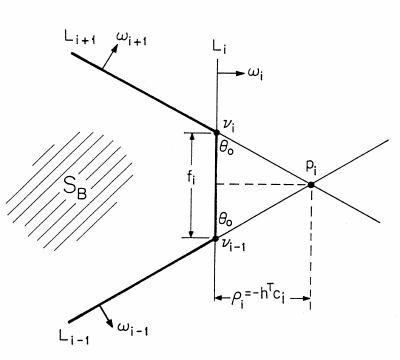
\includegraphics[width=10cm]{images/dicrete-radius-curvature.jpg}
    \caption{Иллюстрация к понятию дискретной кривизны.}
    \label{dicrete-radius-curvature}
\end{figure}

Далее в авторы развивают идею \textbf{дискретного радиуса кривизны} -- величины,
характеризующей гладкость поверхностей главных целей. Представим, что на
рисунке \ref{dicrete-radius-curvature} некоторая материальная точка движется
вдоль $i$-ой стороны многоугольника от экстремальной точки $\nu_{i - 1}$ до
другой экстремальной точки $\nu_{i}$. Тогда во время этого движения вектор
внешней нормали к поверхности меняет угол наклона на величину
$\theta_{0} = \theta_{i} - \theta_{i - 1}$. При этом точка преодолевает
расстояние, равное $f_{i}$. По аналогии с обычным радиусом кривизны,
определяемом как скорость заметания дуги радиусом-вектором поверхности по
отношению к углу наклона радиуса-вектора, авторы определяют дискретный радиус
кривизны как

$$
r_{i} = \frac{f_{i}}{\theta_{0}}
$$

Из геометрических соображений можно показать, что расстояние от точки $p_{i}$
до прямой $L_{i}$ равно $\rho_{i} = -h^{T} c_{i}$, где $c_{i}$ -- $i$-й столбец
матрицы $C$, а из простого тригонометрического соотношения следует, что

$$
f_{i} = \frac{2 \rho_{i}}{tg \theta_{0}}
$$

и, следовательно,

$$
\rho_{i} = \frac{1}{2} r_{i} \theta_{0} tg \theta_{0}
$$

Отсюда следует, что вектор $\rho = - h^{T} C$ состоит из элементов,
пропорциональных дискретным радиусам кривизны $r_{i}$. При этом малые по
величине элементы этого вектора соответствуют "острым" углам, а большие --
"гладким". В дальнейшем авторы статьи испольуют это соображение в целях
коструирования объекта, гладкость которого известна заранее.

\subsubsection{Общие замечания об алгоритмах восстановления}

Всего Prince и Willsky приводят в статье 3 алгоритма для реконструкции выпуклого
тела по измерениям его опорной функции. При этом предполагается, что измерения
опорной функции получаются как

$$
y_{i} = h_{i} + n_{i}, i = 1, \ldots, M
$$

где $h_{i}$ -- точные значения опорной функции, для которых требуется построить
оценку, а $n_{i}$ -- статистические погрешности, которые представляют собой

\begin{enumerate}
 \item Либо независимые одинаково распределенные гауссовы величины с нулевым
 средним и дисперсией $\sigma^{2}$
 \item Либо независимые случайные величины, равномерно распределенные на отрезке
 $[ - \gamma, \gamma]$.
\end{enumerate}

Вследствие наличия статистических погрешностей измерений нельзя утверждать, что
набор $y = (y_{1}, \ldots, y_{M})$ представляют из себя согласованный набор
опорных чисел. Поэтому первой задачей всех алгоритмов является построение
согласованного набора. Следующей задачей является построение такого
согласованного набора, который бы наилучшим образом соответствовал заранее
известной информации об измеряемом объекте.

\subsubsection{Алгоритм ближайшего набора}

\textbf{Алгоритм ближайшего набора} представляет из себя следующее. В данном
случае предполагается, что статистические погрешности представляют собой
гауссовы величины. В случае, когда отсутствует какая-либо информация об
оцениваемом объекте, следует строить оценку максимального правдоподобия вектора
$h$ по вектору измерений $y$ при условии, что $h \in \mathfrak{C}$:

$$
\widehat{h}_{C} = \widehat{h}_{ML} =
\operatornamewithlimits{argmax}_{h: h^{T} C \leq 0}
( - \frac{1}{2} (y - h)^{T} (y - h))
$$

Очевидно, что данная оценка предоставляет такой вектор $h$ из множества
$\mathfrak{C}$, который является наиболее близким к вектору измерений $y$ в
смысле евклидовой метрики. Если $y \in \mathfrak{C}$, то $\widehat{h}_{C} = y$,
в противном случае оценка $\widehat{h}_{C}$ может быть найдена методами
квадратичного программирования.

\subsubsection{Минимаксный алгоритм}


\textbf{Минимаксный алгоритм} предназначен для построения
оценки тела в случае, если заранее известно, что оно представляет из себя тело
с гладкой повехностью. Для этого строится такая оценка, которая
\textit{максимизирует минимальный радиус кривизны} тела. В такой формулировке
решение всегда будет неограниченным, поскольку многоугольники, вписанные в
концетрические окружности неограниченно возратающего радиуса, имеют
неограниченный дискретный радиус кривизны. Эту проблему можно решить, если
предположить, что статистические погрешности равномерно рапределены на отрезке
$[ - \gamma, \gamma]$. В таком случае каждый реального вектора не может
отстоять от измеренной величины больше чем на $\gamma$. Из этого следует, что
реальный вектор и, следовательно, вектор оценки должен содежаться в гиперкубе

$$
\mathfrak{B} = \{h \in \mathbb{R}^{M} |
y - [\gamma, \gamma, \ldots, \gamma]^{T} \leq h \leq
y + [\gamma, \gamma, \ldots, \gamma]^{T}\}
$$

Таким образом, поскольку величины $\rho_{i} = - h^{T} c_{i}$ пропорциональны
дискретным радиусам кривизны $r_{i}$, авторы статьи определяют минимаксную
оценку как

$$
\widehat{h}_{MM} =
\operatornamewithlimits{argmax}_{h \in \mathfrak{C} \cap \mathfrak{B}}
\min_{i = 1, \ldots, M} ( - h^{T} c_{i})
$$

Решение этой задачи оптимизации может быть получено путем применения методов
линейного программирования. Чтобы показать это, введем новую скалярную величину,
удовлетворяющую следущим неравенствам:

$$
\mu \leq - h^{T} c_{i}, i = 1, \ldots, M
$$

Затем рассмотрим расширенные векторы
$u = \left(
\begin{array}{c}
 h_{1} \\
 h_{2} \\
 \vdots \\
 h_{M} \\
 \mu \\
\end{array}
\right)$ и
$ b = \left(\begin{array}{c}
 0 \\
 0 \\
 \vdots \\
 0 \\
 1 \\
\end{array}
\right)$.

В таких обозначениях нетрудно заметить, что исходная задача может
быть переформулирована как максимизация величины $u^{T} b$ относительно
ограничений $\mu \leq - h^{T} c_{i}, i = 1, \ldots, M$. В такой формулировке и
функционал и неравенства ограничений линейны и, следовательно, задача
максимизации может быть решена методами линейного программирования.

Данный алгоритм наделен одним неудачным свойством: как это часто случается при
применении линейного программирования, решение задачи может быть не
единственным. Очевидно, что, например, прибаление произвольного вектора из ядра
$\mathfrak{N}$ матрицы $C$ не изменяет дискретные кривизны объекта и
следовательно, и функционал, максимизирумый в алгоритме. Следовательно, можно
утверждать, что решением задачи нахождения максиминной оценки является целое
семейство объектов, полученных из исходного методом плоскопараллельных сдвигов в
$\mathbb{R}^{2}$. Минимаксная оценка привязана к величинам, полученным из
измерений только внутри гиперкуба $\mathfrak{B}$, и поэтому при увеличении
$\gamma$ полученная минимаксная все меньше зависит от полученных из эксперимента
данных.

Поэтому минимаксный алгоритм всегда стремится построить многоугольник
наибольшего размера в рамках допустимого гиперкуба, причем этот многоугольник
всегда стремится к окружности. Такие результаты получаются даже если истиннное
тело не обладает такими свойствами. Этот недостаток алгоритма послужил для
авторов статьи мотивацией к разработке еще одного алгоритма.

\subsubsection{Минимаксный алгоритм ближайшего набора}

\textbf{Минимаксный алгоритм ближайшего набора} изначально задуман таким
образом, чтобы скомбинировать алгоритм ближайшего набора и минимакный алгоритм.
Сделано это с целью, чтобы получаемая оценка с одной стороны максимально точно
приближала данные, полученные из измерений (как в первом алгоритме), а с другой
-- чтобы учесть заранее известные об объекте данные (как во втором алгоритме).
Идея метода предельно проста: максимизируемый функционал строится как выпуклая
комбинация функционалов двух алгоритмов. С точки зрения статистики алгоритм
представляет собой построение максимальной апостериорной оценки, при этом
слагаемое из алгоритма ближайшего набора играет роль логарифма плотности
измерений (TODO: разобраться в этих понятиях), а слагаемое из минимаксного
алгоритма играет роль логарифма первичной плотности.

Слагаемые берутся с коэффициентами соответственно $\alpha$ и $1 - \alpha$ для
того чтобы дать возможность для настройки алгоритма:

$$
\widehat{h}_{CM} =
\operatornamewithlimits{argmax}_{h \in \mathfrak{C} \cap \mathfrak{B}}
(\alpha f_{C}(h) + (1 - \alpha) f_{M}(h))
$$

где $0 \leq \alpha \leq 1$ и $f_{C}(h)$ и $f_{M}(h)$ представляют из себя
функционалы из первых двух алгоритмов:

$$
f_{C}(h) = - \frac{1}{2} (y - h)^{T} (y - h)
$$

$$
f_{M}(h) = \min_{i = 1, \ldots, M} (- h^{T} c_{i})
$$

Решение данной задачи может быть найдено методами квадратичного
программирования путем расширения вектора $h$, как это было сделано в
минимаксном алгоритме. Заметим, что поскольку $\alpha \neq 0$, условие
принадлежности гиперкубу $\mathfrak{B}$ может быть опущено и решение задачи
является единственным.

\subsubsection{Модификация алгоритмов, учитывающая информацию о абсолютном
положении объекта}

Предположим, что заранее известно, что центр масс вершин некоторого объекта
расположен в точке $\overline{\nu}$. Тогда данная информация может быть также
заложена в процесс восстановления многоугольника -- восстановленный
многоугольник должен обладать таким же свойством. Данное условие может быть
достигнуто просто путем расширения набора ограничений еще одним линейным
равенством:

$$
N^{T} h = \frac{M}{2} \overline{\nu}
$$

Вследствие линейности данного уравнения внесение его в число ограничений любого
из трех введенных выше алгоритмов не внесет качественных изменений в методы
работы этих алгоритмов (линейное и квадратичное программирование). Эффект от
добавления такого ограничения может быть довольно заметным.

\newpage
\subsection{Методы восстановления многоугольников и их приложения к
задаче распознания цели по данным лазерного радара (по статье Lele, Kulkarni,
Willsky)}

Дальнейшее развитие рассматриваемая проблема нашла в исследовании авторов Lele,
Kulkarni и Willsky, которое было описано в статье
\cite{journals/josaa/LeleKW92}. Более подробную информацию можно найти в
дипломной работе Lele \cite{thesis/Lele90}.

Данное исследование охватывает совершенно новую область применения --
распознание формы объектов по данным лазерного радара. В ней описано обобщение
первый алгоритма ближайшего набора Prince и Willsky для случая, когда
направления, по которым производится измерение опорной функции, распределены
произвольным образом. Также в ней вводится 2 новых алгоритма, которые позволяют
строить тело на основе априорной информации о количестве его сторон и
либо направлениях нормалей этих сторон, либо об относительных углах между этими
направлениями.

\subsubsection{Воосстановление многоугольника со сторонами по углам измерения}

Данный алгоритм является обобщением алгоритма ближайшего набора из статьи Prince
и Willsky, в котором тело строится по конечному набору величин
$y_{1}, y_{2}, \ldots, y_{M}$,  которын представляют собой измеренные с
погрешностями значениями опорной функции по направлениям вдоль известных углов
$\theta_{1} < \theta_{2} < \ldots < \theta_{M}$, которые называются
\textbf{углами измерения}. Отличие от упомянутого алгоритма состоит в том, что
критерий матрица в неравенстве из критерия согласованности записывается
несколько иным образом.

Тройка опорных чисел $h_{i - 1}, h_{i}, h_{i + 1}$ по углам $\theta_{i - 1},
\theta_{i}, \theta_{i + 1}$ являтся согласованной тогда и только тогда, когда
выполнено следующее неравенство:

$$
h_{i - 1} sin(\theta_{i + 1} - \theta_{i}) -
h_{i} sin(\theta_{i + 1} - \theta_{i - 1}) +
h_{i + 1} sin(\theta_{i} - \theta_{i - 1}) \geq 0
$$

Опорная теорема теперь записывается следующим образом:



\begin{flushleft}
 \textbf{Теорема 3.} \textbf{Обобщенная двумерная опорная теорема}.
 Набор действительных чисел
 $h = (h_{1}, h_{2}, \ldots, h_{M}) \in \mathfrak{R}^{M}$
 является набором опорных чисел по направлениям вдоль углов
 $\theta_{1} < \theta_{2} < \ldots < \theta_{M}$ тогдя и только тогда, когда
 выполнено следующее матричное неравенство:

 $$
 C h \geq 0
 $$
 
 гдк матрица $C$ представляет собой следующее:

  $$
 \left(
 \begin{array}{ccccccc}

\scriptstyle     -sin(\theta_{2} - \theta_{M}) &
\scriptstyle     sin(\theta_{1} - \theta_{M}) &
\scriptstyle     0 &
\scriptstyle     \ldots &
\scriptstyle     0 &
\scriptstyle     0 &
\scriptstyle     sin(\theta_{2} - \theta_{1}) \\

\scriptstyle      sin(\theta_{3} - \theta_{2}) &
\scriptstyle      -sin(\theta_{3} - \theta_{1}) &
\scriptstyle      sin(\theta_{2} - \theta_{1}) &
\scriptstyle      \ldots &
\scriptstyle      0 &
\scriptstyle      0 &
\scriptstyle      0 \\

\scriptstyle      0 &
\scriptstyle      sin(\theta_{4} - \theta_{3}) &
\scriptstyle      -sin(\theta_{4} - \theta_{2}) &
\scriptstyle      \ldots &
\scriptstyle      0 &
\scriptstyle      0 &
\scriptstyle      0 \\

\scriptstyle      \vdots &
\scriptstyle      \vdots &
\scriptstyle      \vdots &
\scriptstyle      \ddots &
\scriptstyle      \vdots &
\scriptstyle      \vdots &
\scriptstyle      \vdots \\

\scriptstyle      0 &
\scriptstyle      0 &
\scriptstyle      0 &
\scriptstyle      \ldots &
\scriptstyle      -sin(\theta_{M - 1} - \theta_{M - 3}) &
\scriptstyle      sin(\theta_{M - 2} - \theta_{M - 3}) &
\scriptstyle      0 \\

\scriptstyle      0 &
\scriptstyle      0 &
\scriptstyle      0 &
\scriptstyle      \ldots &
\scriptstyle      sin(\theta_{M} - \theta_{M - 1}) &
\scriptstyle      -sin(\theta_{M} - \theta_{M - 2}) &
\scriptstyle      sin(\theta_{M - 1} - \theta_{M - 2}) \\

\scriptstyle      sin(\theta_{M} - \theta_{M - 1}) &
\scriptstyle      0 &
\scriptstyle      0 &
\scriptstyle      \ldots &
\scriptstyle      0 &
\scriptstyle      sin(\theta_{1} - \theta_{M}) &
\scriptstyle      sin(\theta_{1} - \theta_{M - 1}) \\
 \end{array}
 \right)
 $$
\end{flushleft}


\newpage
\section{Предлагаемый подход}

\newpage
\bibliographystyle{plain}
\bibliography{references}

\end{document}
